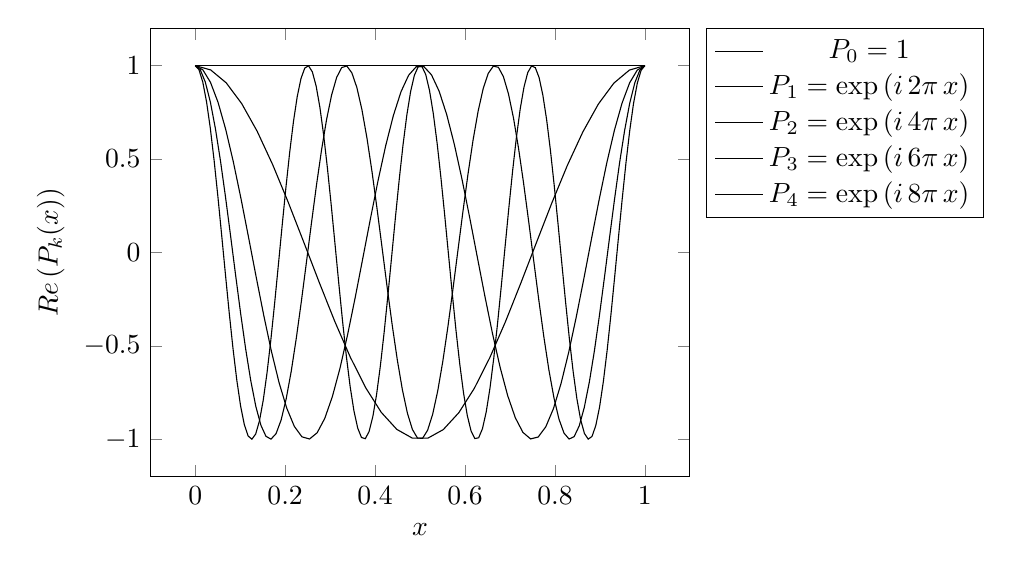
\begin{tikzpicture}
\begin{axis}[
  xlabel=$x$,
  ylabel=$\operatorname{Re}\left(P_k(x)\right)$,
  legend pos=outer north east]
\addplot[samples=2, domain=0:1] {1};
\addlegendentry{$P_0 = 1$};

\addplot[samples=30, domain=0:1] {cos(deg(6.28*x))};
\addlegendentry{$P_1 = \exp\left(i \, 2\pi \, x\right)$};

\addplot[samples=60, domain=0:1] {cos(deg(2*6.28*x))};
\addlegendentry{$P_2 = \exp\left(i \, 4\pi \, x\right)$};

\addplot[samples=90, domain=0:1] {cos(deg(3*6.28*x))};
\addlegendentry{$P_3 = \exp\left(i \, 6\pi \, x\right)$};

\addplot[samples=120, domain=0:1] {cos(deg(4*6.28*x))};
\addlegendentry{$P_4 = \exp\left(i \, 8\pi \, x\right)$};
\end{axis}
\end{tikzpicture}